\newcommand{\tauconst}{5000}
\newcommand{\query}{[INSERIRE LA QUERY CON NOTAZIONE CTL]}
\newcommand{\mT}{\ensuremath{\mu_T}}
\newcommand{\vT}{\ensuremath{\sigma_T}}
\newcommand{\mH}{\ensuremath{\mu_H}}
\newcommand{\vH}{\ensuremath{\sigma_H}}
\newcommand{\K}{\ensuremath{K}}
\newcommand{\expdel}{\ensuremath{\lambda}}

\section{Properties}
In this section we are going to describe the properties that we have verified over the system to ensure its correctness and to analyse its behaviour. Unless otherwise specified, we ran our verifications with a time bounded to \tauconst \space time units, in order to emulate a realistic environment when fully operational.

We have reported two verifications, as we considered them crucial for analysing the behaviour of our system. The first one, described at section \ref{podsunavailable}, has been performed with the aim of investigating the probability of running out of pods available in the grid. The second one aims at analysing the probabilities of running out of space in the task queue, during an execution.

During the verification phase we have used the default statistical parameters of \UPPAAL. It is reasonable to consider a confidence of the 95\% for verification purposes, as well as the other values already present by default inside the tool, since a simplified model would not need higher statistical accuracy. The parameters with the respective values are reported in the Table \ref{tab:statparam}.

\begin{table}[h]
    \centering
        \begin{tabular}{|c c|} 
            \hline
            Parameter & Value \\ [0.5ex] 
            \hline\hline
            $\pm\delta$ & 0.01 \\
            $\beta$ & 0.05 \\
            $\alpha$ & 0.05 \\
            $\epsilon$ & 0.05 \\
            $\mu_0$ & 0.9 \\
            $\mu_1$ & 1.1 \\
            Trace resolution & 4096 \\
            Discretization step & 0.01 \\ [0.5ex] 
            \hline
        \end{tabular}
        \caption{Statistical parameters of \UPPAAL}
        \label{tab:statparam}
\end{table}

\subsection{Pods unavailable} \label{podsunavailable}
This property has been generally analysed, without entering in the details of each single configuration.

We analysed two cases and observed the reaction of the system in each of them.

Considering that the pods could become unavailable when 
\begin{equation} \label{podsavailable}
    PODS\_NUMBER < QUEUE\_LENGTH + ROBOTS\_NUMBER
\end{equation}
we considered a case in which this formula is respected, and another one in which is not. Modifying the grid layout or the grid dimensions the number of pods can vary. Hence, we changed the grid dimension accordingly with our necessities.

To verify this property we checked if the template \emph{Task\_queue} eventually enters the state \emph{task\_queue.pods\_unavailable}. The formula can be found in the tab \emph{Verifier} of \UPPAAL. The equivalent CTL formula is:
\begin{equation}
    SOSTITUIRE ->  \lnot \square \vee \vdash \lozenge \wedge \models  <- SOSTITUIRE
\end{equation}
Where $TAU (= \tauconst)$ is the upper bound limit.
\\

In the first case, we used a \texttt{6x6} grid. This configuration respects the equation \ref{podsavailable}. As the Table \ref{tab:tabpodsunavailable} shows, it's quite sure that the system fails [DICO MEGLIO, PRECISO ANCHE IL NUMERO DI RUNS]. It was expected.
\\

In the second case, we used a \texttt{10x10}, thus violating the equation \ref{podsavailable}. In the Table \ref{tab:tabpodsunavailable} we can see that in this case, the probability is the inverse of the previous one, with even less runs necessary. In fact, it should be impossible to reach the state \emph{task\_queue.pods\_unavailable} when the equation is not respected (29 runs is the minimum in \UPPAAL) [ANCHE QUI SCRIVERLA MEGLIO].

\begin{table}[h]
    \centering
        \begin{tabular}{| c || c c |} 
            \hline
             & First configuration & Second configuration \\ [0.5ex] 
            \hline\hline
            Grid dimension & \texttt{6x6} & \texttt{10x10} \\
            Number of runs & 54 & 29 \\
            \hline\hline
            $prob \in$ &  $[90.11\%,99.95\%]$ & $[0\%,0.098\%]$\\ [0.5ex] 
            \hline
        \end{tabular}
        \caption{Scenario 1 table [NAME]}
        \label{tab:tabpodsunavailable}
    \end{table}

\subsection{Full queue [UN NOME FIGO PER IL TITOLO?]}
This is the most important property to be verified, in order to understand if the system reacts in a proper way to several configurations. The system should sustain a high number of tasks generated during the execution.

In this section we will stress the system by changing the delays and the grid configuration. We will also try adding some robots into the system, so that we will be able to see the main differences, comparing them and understanding what are the trade-off to take into account. In particular, the parameters which I will refer to are listed here:
\begin{itemize}
    \item \mT: the average delay of the task generation
    \item \vT: the standard deviation of the task generation
    \item \mH: the average delay when a human picks an item
    \item \vH: the standard deviation when a human picks an item
    \item \K: the \emph{deterministic} value of the time that passes between each move of the robot
    \item \expdel: the delay with which the robot claims a task. Note that this parameter has not been changed in any configuration, as we considered $\expdel= 1$ a realistic situation [MIGLIORARE FRASE].
\end{itemize}

We analysed three different scenarios. In the first one, we analysed the behaviour og the system with a \texttt{10x10} grid and 3 robots. In the second one, we increased the number of robots to 6, maintaining the same grid dimension. Finally, we observed how the system reacts to a \texttt{8x12} grid, being it rectangular and not squared. In this case, we used 4 robots, to simulate an average situation [?].

We considered the length of the queue to be always equal to 20 maximum tasks. The variable parameter was the frequency, not the length [MI E' VENUTO IN MENTE ALL'ULTIMO POI LO SISTEMO].

For all the scenarios we used the same query, that can be found in the tab \emph{Verifier} of \UPPAAL. It is equivalent to the CTL formula:

\begin{equation}
    SOSTITUIRE ->  \lnot \square \vee \vdash \lozenge \wedge \models  <- SOSTITUIRE
\end{equation}
Where $TAU$ is the upper bound limit. As I mentioned before, $TAU = \tauconst$ in each verification.

In order to offer a general overview of all the vericiations, we collected all the results in the Table \ref{tab:scenonetable}. We will use this table during the description of each scenario, describing why we used certain values and the purpose of each verification.

\begin{table}[hb]
    \centering
        \begin{tabular}{| c || c c c c c |} 
            \hline
            \texttt{10x10} & Scen 1.a & Scen 1.b & Scen 1.c & Scen 1.d & Scen 1.e \\ [0.5ex] 
            \hline\hline
            \mT & 40 & 150 & 40 & 30 & 30 \\
            \vT & 5 & 10 & 5 & 5 & 5 \\
            \mH & 3 & 6 & 6 & 3 & 6 \\
            \vH & 2 & 4 & 4 & 2 & 4 \\
            \K & 1 & 1 & 2 & 1 & 1 \\
            \expdel & 1 & 1 & 1 & 1 & 1 \\
            \hline\hline
            $p[\%]\in$ &  $[24.8,34.8]$ &  $[4.14,14.1]$ &  $[90.2,100]$ & $[76.4,86.4]$ & $[90.2, 100]$ \\ [0.5ex] 
            \hline
        \end{tabular}
        \caption{Scenario 1 table [NAME]}
        \label{tab:scenonetable}
    \end{table}


\begin{table}[hb]
    \centering
        \begin{tabular}{| c || c c c |} 
            \hline
            \texttt{10x10} & Scen 2.a & Scen 2.b & Scen 2.c \\ [0.5ex] 
            \hline\hline
            \mT & 40 & 150 & 200 \\
            \vT & 5 & 10 & 10 \\
            \mH & 3 & 6 & 6 \\
            \vH & 2 & 4 & 4\\
            \K & 1 & 1 & 1 \\
            \expdel & 1 & 1 & 1 \\
            \hline\hline
            $p[\%]\in$ &  $[60.2,70.2]$ &  $[20.0,30.0]$ &  $[6.19,16.2]$ \\ [0.5ex] 
            \hline
        \end{tabular}
        \caption{Scenario 2 table [NAME]}
        \label{tab:scentwotable}
\end{table}

\subsubsection{First Scenario} \label{firstscenario}
The first scenario is the simplest one. In this case, there were 3 robots and the dimension of the grid was \texttt{10x10}.

Given that three robots are not able to handle a large number of tasks, we firstly chose to give a high average time for the task generation delay (\mT) while maintaining a general realistic behaviour between the robots and the human (\mH). We assumed that the human is slower than the robots and that it has a significant high deviation standard (\vH). We also assumed the task generation to be quite constant, keeping a small deviation standard (\vT), in order to avoid creating a too floating situation. All these parameters are collected in the scenario \emph{Scenario 1.a} of the Table \ref{tab:scenonetable}.

The aforementioned assumptions could bring to the conclusion that, probably, the robots will be able to handle the tasks generated quite easily. However, the verification results show that there is about the 30\% of probability that the queue will reach the maximum size.
\\

As a consequence, we decreased the task generation frequency until the result reached a low probability. We did that to understand what is, in this configuration, the maximum frequency that the system can handle.

In these scenario we focused on the average delay time \mT \space and we changed the other parameters only in order to give a realistic behaviour to the overall system. [DEVO CAPIRE COME SPIEGARE BENE IL MOTIVO PER CUI ABBIAMO SOLO CAMBIATO \mT]

We used the values indicated at Table \ref{tab:scenonetable} under \emph{Scenario 1.b} and we considered the resulting interval sufficient to indicate $\mT = 150$ as the maximum frequency [NON MI PIACE LA FRASE, praticamente ho spiegato che grazie a quel range di probabilità, a noi va bene così].
\\

Finally, we tried stressing the system in order to understand when it can no more handle the situation. We did it in three ways:
\begin{itemize}
    \item Firstly, we tried increasing \K, with the aim of delaying the robots. It was enough to double the delay in order to reach the maximum probabilistic range as shown at Table \ref{tab:scenonetable} under \emph{Scen 1.c}.
    \item Subsequently we tried decreasing the task generation delay. At Table \ref{tab:scenonetable} under \emph{Scen 1.d}, we can see that, just decreasing the generation delay by $10$, the probabilistic range increased of about the $50\%$ with respect to the \emph{Scen 1.a}.
    \item Finally, we modified the previous analysis. We kept the same values, except for delaying a little the human (Table \ref{tab:scenonetable}, \emph{Scen 1.e}). It is enough to delay the human some time units in order to reach the maximum possible range.
\end{itemize}

In conclusion, we would like to underline the main characteristics identified in the first scenario. We can notice that, in order to stress the system, decreasing a few time units the task generation delay is enough to have the system unable to handle the configuration. The same can be said for increasing the human delay.

On the other hand, the system begins to behave in a smooth way only when we set quite high the task generation delay. We will better understand in section \ref{secondscenario} that this behaviour is typical when there are few robots in the system.

\subsubsection{Second Scenario} \label{secondscenario}
In this scenario, we will analyse a configurations with six robots and a \texttt{10x10} grid.

The intuitive reasoning could be that the more robots there are in the system, the smoothest it will be in handling a non trivial number of tasks. Moreover, it should be improbable for the robots to find `traffic' in the map, as they are much less than the total number of cells available.

However, the results of the verification are worser than the expected. In order to compare the two scenarios, we used the same values of the \emph{Scen 1.a} at Table \ref{tab:scenonetable}. The resulting probability is shown at Table \ref{tab:scentwotable} at \emph{Scen 2.a}. We can observe that the probability of filling up the queue is $35\%$ higher than the one of \emph{Scen 1.a}.
\\

Subsequently, we proceeded in the same way as in section \ref{firstscenario}, as shown in \emph{Scen 2.b} and \emph{Scen 2.c} of Table \ref{tab:scentwotable}. Comparing \emph{Scen 2.b} with \emph{Scen 1.b} underlines that the resulting probability of the former is $15\%$ higher than the probability of the latter. However, we can notice that the gap between the two configurations has decreased from $30\%$ to $15\%$. As we mentioned at the end of section \ref{firstscenario}, increasing the number of robots eases la velocità con cui si abbassa la probabilità, quindi la smoothness del sistema [OCHO QUA SI DEVE SCRIVERE BENE].
\\

Finally, we tried finding the maximum frequency that allows us considering the system stable and smooth, as we did in section \ref{firstscenario}. \emph{Scen 2.c} shows the results of a verification with $\mT = 200$. We can consider this result acceptable from the point of view of the smoothness of the system.
\\

In conclusion, we can observe that there is a trade-off to be taken into account. More robots are able to handle more tasks in a more efficient way. However, depending on the grid configuration, they could obstruct each other and worsen the overall efficiency.

\begin{table}[b]
    \centering
        \begin{tabular}{| c || c c c c |} 
            \hline
            \texttt{12x8} & Scen 3.a & Scen 3.b & Scen 3.c & Scen 3.d \\ [0.5ex] 
            \hline\hline
            \mT & 40 & 40 & 40 & 40 \\
            \vT & 5 & 80 & 5 & 5 \\
            \mH & 3 & 3 & 6 & 6 \\
            \vH & 2 & 2 & 2 & 15\\
            \K & 1 & 1 & 1 & 1 \\
            \expdel & 1 & 1 & 1 & 1 \\
            \hline\hline
            $p[\%]\in$ &  $[12.7,29.1]$ &  $[7.87,22.4]$ &  $[16.9,34.7]$ &  $[27.6,47.2]$ \\ [0.5ex] 
            \hline
        \end{tabular}
        \caption{Scenario 2 table [NAME]}
        \label{tab:scenthreetable}
\end{table}

\subsubsection{Third Scenario}
The last scenario that we would like to present is less specific. We stressed an environment with a \texttt{12x8} grid, as shown in Figure \ref{fig:grid12x8} and 4 robots, in order to analyse the behaviour of the system in a rectangular grid. 

\begin{figure}
    \centering
    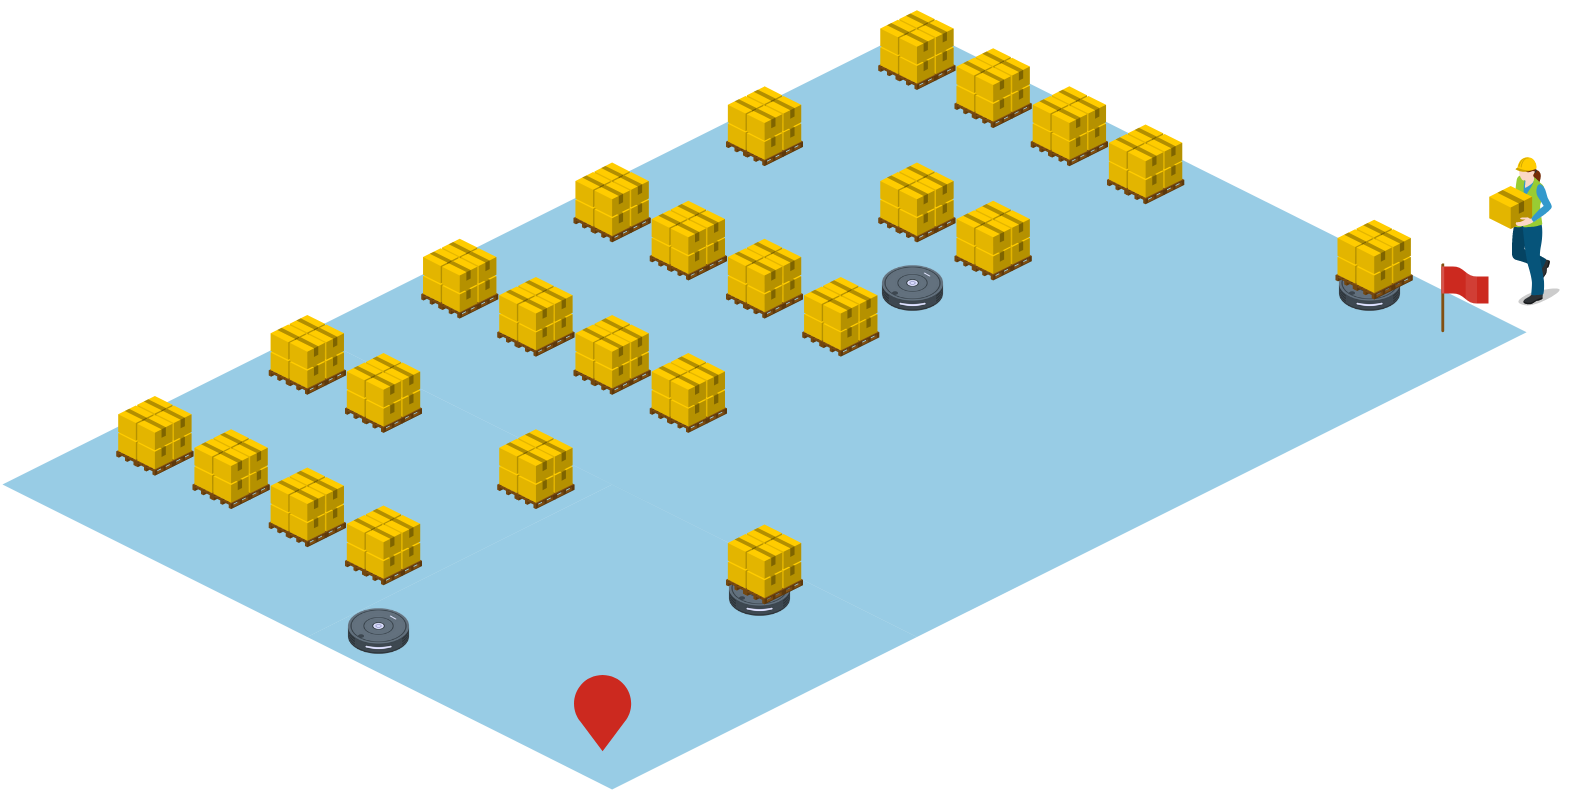
\includegraphics[width=0.75\textwidth]{resources/grid12x8.png}
    \caption{12x8 grid layout}
    \label{fig:grid12x8}
\end{figure}

Here we concentrated more on the reactions of the system when changing the standard deviations (\vH \space and \vT) and the human average delay time (\mH).

The relevant results are collected at Table \ref{tab:scenthreetable}. We began analysing the system in a realistic environment (\emph{Scen 3.a}) and then we changed the relevant parameters. We isolated the analysis for each parameter, changing only one value at a time, in order to ease the behavioural evaluation.

In the first place, we analysed the system reaction in a standard and realistic situation, as it is shown at \emph{Scen 3.a}. The resulting probabilistic interval is quite low, as it floats around the $20\%$, but it is not sufficient for considering the system smooth in this configuration.

We subsequently stressed the environment in three different ways:
\begin{itemize}
    \item Firstly, we increased \vT. We tried several values to see how the system reacts to them, and we understood that the system actually responds when the standard deviation is a lot greater than the average (in this case, \mT). Hence, it reacts with a significant difference when the actual delay changes a lot at each iteration. \emph{Scen 3.b} at Table \ref{tab:scenthreetable} highlights this behaviour, even though the gap is not as big as if we were increasing \mT.
    \item Secondly, we tried increasing \mH, simulating a situation in which the human is much slower than the robot. As expected, it results in an increase of the resulting probability. The human appears to be an important member of the production line. The result is detailed at Table \ref{tab:scenthreetable}, \emph{Scen 3.c}.
    \item Finally, we increased \vH while maintaining the \emph{Scen 3.c} parameters (Table \ref{tab:scenthreetable}, \emph{Scen 3.d}). As in the previous cases, the general expected behaviour is respected and the probability range increases.
\end{itemize}

In conclusion, we have noticed that the standard deviation impacts less the system rather than the average delay. This was expected, even though this verification has been very useful in order to understand the numerical differences between deviation and average.